% This work is licensed under the Creative Commons
% Attribution-NonCommercial 3.0 Unported License. To view a copy of this
% license, visit http://creativecommons.org/licenses/by-nc/3.0/.
\section{Versuchsaufbau und Durchführung}

\subsection{Helium-Neon-Laser}
Der HeNe-Laser ist ein Gaslaser mit einem Gemisch aus He- und Ne-Atomen
im Verhältnis 5 zu 1 bei einem Druck von etwa \SI{1}{Torr}, was in etwa
\SI{133.3224}{Pa} entspricht.  Die Besetzungsinversion wird über
eine Gasentladung erreicht.  Am Anfang und Ende des Laserrohres, in dem
das Gas eingeschlossen ist, befinden sich \name{Brewster}-Fenster, um 
einen möglichst verlustfreien Durchlaß von Licht zu ermöglichen.  Die Fenster
sind im \name{Brewster}-Winkel zur Strahlrichtung ausgerichtet, so dass
nur die s-polarisierte Komponente teilweise reflektiert wird (siehe
\cref{fig:brewster-window}.  Dadurch wird das Laserlicht p-polarisiert
und kann ohne Verlust die Fenster passieren. Von den beiden Gasen 
funktioniert das Helium als Pumpgas, das die Energie durch Entladung 
aufnimmt und
dann an die Neonatome über Stöße weiterreicht.  
Neon ist also das eigentliche
Lasermaterial.  Lasertätigkeit kann auf mehreren Linien beobachtet
werden, wobei die rote Linie mit $\lambda = \SI{632.8}{nm}$ am
intensivsten ist.  Für diese Linie ist der Übergang von 3s zu 2p in Neon
verantwortlich (siehe \cref{fig:laser-schema}).

\begin{figure}[h]
  \centering
  \includegraphics[width=0.5\textwidth]{figures/Brewster_window}
  \caption{Zur Funktionsweise eines Brewsterfensters. Nur die 
    Komponente des Lichtes, welche parallel zur Einfallsebenen liegt, 
    wird 
    durchgelassen. Die andere Komponente wird reflektiert. 
    Die Abbildung ist aus
    der englischen Wikipedia entnommen \cite{wikipedia:brewster_angle}
    und ist unter der Creative Commons Attribution-Share Alike 3.0
    Unported lizensiert.}
  \label{fig:brewster-window}
\end{figure}

\begin{figure}
  \centering
  \includegraphics[width=0.8\textwidth]{figures/HeNe-Laser}
  \caption{Der grundlegende Aufbau des HeNe-Lasers.  Die Abbildung ist
    aus der deutschen Wikipedia entnommen \cite{wikipedia:laser} und ist
    unter der GNU Free Documentation License, Version 1.2 lizensiert.}
  \label{fig:laser}
\end{figure}

\subsection{Aufbau der Apparatur}
Auf einer Schiene befestigt sind ein Justierlaser (Wellenlänge
\SI{532}{nm} mit reduzierter Leistung von \SI{0.2}{mW}), die
Resonatorspiegel, das Laserrohr und Beugungsblenden mit Fadenkreuz.  Das
Laserrohr ist mit einem HeNe-Gemisch gefüllt, ist ca. \SI{408}{mm} lang und 
hat einen Durchmesser von \SI{1.1}{mm}.  Als Resonatorspiegel stehen
vier verschiedene Spiegel mit Durchmessern von je \SI{12.7}{mm} zur 
Verfügung.
In \cref{fig:laser} ist eine Skizze des Laseraufbaus dargestellt.

\begin{figure}
  \centering
  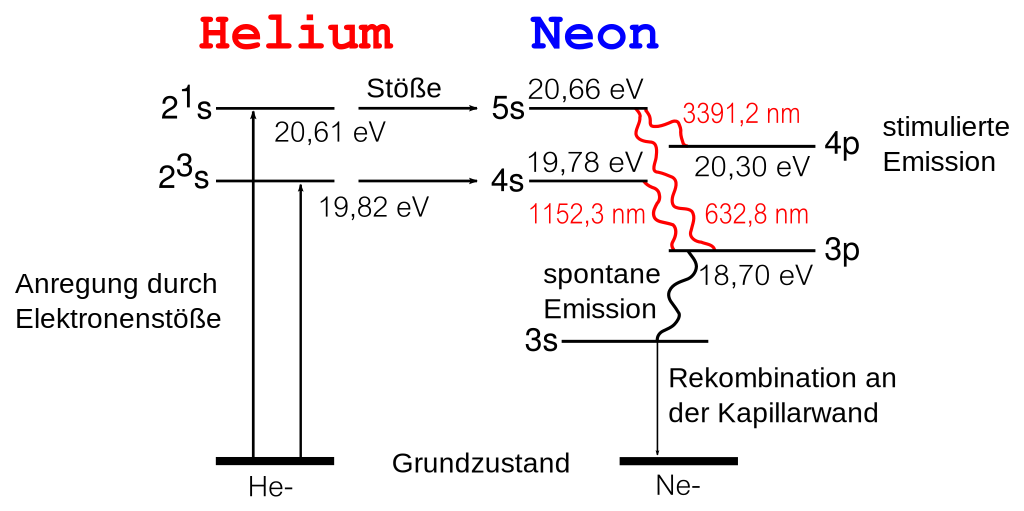
\includegraphics[width=0.8\textwidth]{figures/HeNe-Laser-Energieschema}
  \caption{Das Energie-Schema des HeNe-Lasers.  Die Abbildung ist aus
    der deutschen Wikipedia entnommen \cite{wikipedia:laser} und ist
    unter der Creative Commons Attribution-Share Alike 3.0 Unported
    lizensiert.}
  \label{fig:laser-schema}
\end{figure}

Weiter stehen verschiedene Geräte für die Meßdurchgänge zur Verfügung:
Photo-Dioden und Meßgerät zur Stabilitätsmessung und Modenvermessung,
Beugungsspalt zur Bestimmung der Wellenlänge und Polarisator zur
Bestimmung der Polarisation.  Zum Betrieb des Laserrohrs gibt es eine
Spannungsquelle, die die für die Gasentladung notwendige Hochspannung
liefert.  Da auch die Wellenlänge mit Hilfe eines optischen Gitters
bestimmt werden soll und daher die Lage der Interferenzmaxima bestimmt
werden müssen, befindet sich am Ende im Strahlengang auch ein Schirm.

\subsection{Durchführung}
Mithilfe des Justierlasers und der Beugungsblenden werden zunächst das
Laserrohr und die Resonatorspiegel ausgerichtet.  Danach wird der
Justierlaser ausgeschaltet und am Hochspannungsgenerator ein Strom von
\SI{6.5}{mA} eingestellt.  Jetzt leuchtet das Laserrohr rot, allerdings
dürfte beim Laser noch keine Lasertätigkeit einsetzen.  Durch Justage an
den Stellschrauben der Resonatorspiegel setzt die Lasertätigkeit ein.

Zur Überprüfung der Stabilitätsbedingung wird folgendermaßen
vorgegangen:  Unter Zuhilfenahme der Photodiode, die die Intensität des
Laserlichts mißt, wird der Laser mit den Resonatorstellschrauben auf die
maximale Leistung einjustiert.  Bei laufendem Laser wird jetzt der
Resonatorspiegel verschoben und die Laserleistung nachjustiert.  Die
maximal mögliche Resonatorlänge wird notiert.  Dann wird das Verfahren
für einen weiteren Resonator wiederholt.

Zur Beobachtung von TEM-Moden wird ein dünner Draht als Modenblende
zwischen Laserrohr und Resonatorspiegel gebracht und geeignet
verschoben, so daß auf dem Schirm verschiedene Moden zu sehen sind.
Danach werden die Moden mit der Photodiode vermessen.  Da es uns mit dem
vorhandenen Wolframdraht nicht gelungen ist, eine andere Mode außer der
Grundmode zu isolieren, haben wir ein Haar verwendet.

Zur Polarisationsbestimmung wird ein Polarisator hinter den
teildurchlässigen Resonatorspiegel gestellt und für verschiedene
Polarisatorwinkel die Intensität gemessen.

Um die Wellenlänge des Lasers zu bestimmen, wird ein optisches Gitter
zwischen teildurchlässigen Resonatorspiegel und Schirm gestellt.  Auf
dem Schirm beobachtet man Beugungsmaxima und -minima.  Dann werden die
Abstände der Maxima von der optischen Achse gemessen.
